%*****************************************
\chapter{From tissue to single cell transcriptomics, a paradigm shift}\label{ch:singlecell}
%*****************************************
\section{Spatially referenced single cell-like in-situ hybridization data}
  \subsection*{Dividing images into "cells"}
  Because in-situ hybridization keeps the studied tissue spatially untouched, achieving single cell gene expression resolution from one image obtained through fluorescent microscopy is a matter of microscope performance and cell size. For big enough cells, single cell resolution has been documented as far as 1989 \cite{tautz89} with some work specifically directed towards achieving this single cell resolution \cite{poulsen93}.\\
  
  When considering \cite{Tomer10} dataset, with current microscope technology, achieving single cell level resolution in \platy{}'s brain on one particular image is feasible. However, our main limitation is the quantity of data involved, indeed, each brain is separated into 20 slices, for 169 genes. This technical bottleneck can be overcome with an automated way of analysing the fluorescence images. However this is not an easy task, as the computer program required needs to be able to ``see" and divide the global picture into cells. Considering that all cells do not exhibit the same shape and size, constructing this ``cell model" is a very complicated task.\\
  
  Possibilities exit to highlight the limits of the cells and to automatically acquire those boundaries through computer vision. They rely on targeting proteins in the membrane or in the extracellular matrix of the cells with specific fluorescent probes. Once the boundaries are acquired, defining every cell is a matter of finding enclosed spaces. To that end, numerous contour detection algorithms exist \cite{li95,fan01,arbelaez11}.\\
  
  Unfortunately, a dataset with the cells limits highlighted does not yet exist for \platy{}'s brain, making a precise division of the images into cells very difficult. Instead, Tomer used a basic approach to divided the images, the ``cube" model \cite{Tomer10}.


  \subsection*{A simple cell model, the "cube" data}
  
  Every slice of \platy{}'s brain being aligned onto the reference gene scaffold (see section \ref{sec:gene_expression_lab}) for all 169 genes, the ``cube" model simply consists in dividing each image into square approximately the size of an average cell. In our dataset, the size chosen was 3 \microm{2}. Importantly, this is actually smaller than the average cell size in \platy{}'s brain. each slice of the brain being approximately 3 \microm{} thick, the resulting dataset, referenced on a 3-dimensional axis, will contain 3 \microm{3} cubes, each of those attached to the luminescence data for 169 genes.\\
  
  Of course this cell model is far from perfect, it assumes that every cell in the brain are roughly the same size and cubical, which is clearly not the case. Consequently, the ``cube" model will introduce errors in the dataset. The first type of error occurs within areas where the genes under study are highly expressed. In that case, the florescence my contaminate the cubes around that do not necessarily express the same gene see figure \ref{fig:cubeserrors}A. The second type of error is introduced by the choice of 3 \microm{3} cubes. As they are smaller than the average cell, some cubes will fall on areas that may be artificially empty. Indeed, transcription in the cells mainly happens in the nucleus, mRNA then travel in the cytoplasm to be translated but they are not evenly distributed across the cell, in particular for some large cells, parts of the cytoplasm may record no expression in a cell that actually contains a lot of transcripts, see figure \ref{fig:cubeserrors}B.\\
  
  Hence the data will tend to show some discontinuity and inconsistency spatially. With that fact in mind, any method hat we develop using this data, will have to take into account this spatial discontinuity and try as much as possible to smooth over those potential expression gaps.\\
  
    \begin{figure}[bth]
\centerline{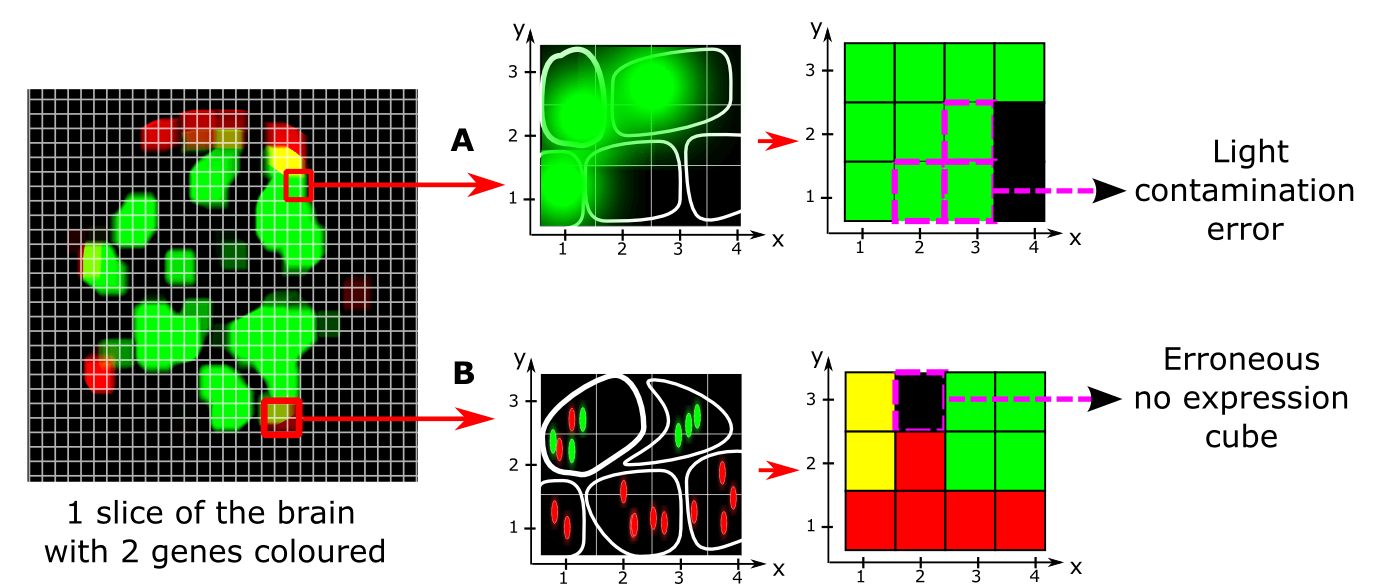
\includegraphics[width=0.9\linewidth]{gfx/chapter2/cubeserrors.png}}
\caption{Errors introduced by the ``cube" cell model. Path A shows how regions with highly expressed genes can introduce errors through light contamination. Path B shows how .}\label{fig:cubeserrors}
	\end{figure}

\section{Singe cell RNA sequencing, building a map of the full transcriptome}
  \subsection*{Sequencing single cell RNA contents}
    - Same as tissue sequencing but with a lot less starting material
    - Present the main techniques used (see with Luis) : Microfluidics and others
    - We obtain the full transcriptome of every cell sequenced

  \subsection*{Mapping back gene expression to a spatial reference}
    - Single cell RNA-seq at the moment does not allow to track cell localization
    - Need to map the transcriptome back to a spatial reference
    - Use in-situ hybridization results as reference


\section{About the quantitative trait of single cell expression data}
  \subsection*{Light contamination in in-situ hybridization data}
    - FIG 5 : show light intensity across one slice
    - Explain problem of scale and light contamination

  \subsection*{Technical noise in single cell RNA-seq data}
    - FIG 6 : show "typical" correlation plot from single cell RNA-seq with the noise increasing when reducing starting material
    - Both methods are currently unreliable quantitatively => need to binarize

\section{Binarizing gene expression datasets}
  \subsection*{Binarizing in-situ hybrdization datasets}
    - With biological knowledge and a limited number of genes
    - Possibility to compare spatially the resulting binary expression patterns to microscope data and adjust for each gene the threshold manually
  \subsection*{Binarizing whole transcriptomes}
    - Manual curation no longer possible
    - Thresholding ideally with density peaks
    - Problems that may occur and possible solutions (figure?)

\section{Preliminary results on mapping single cell RNA-seq data in from Platynereis' brain}
  \subsection*{Single cell RNA-seq in Platynereis' brain}
    - Present the data (number of cell)
    - Present the method used (to dissolve the brain, to capture the cells, to sequence the cells
  \subsection*{Mapping back RNA-seq data back to PrimR in-situ hybridization assays}
    - Select the overlapping genes
    - Present mapping method (Nuno's pipeline)
    - Present simple mapping technique and why it is not satisfactory
    - Present John's method  
    - FIG 6: find a nice way to show a few good examples of mapping

%*****************************************
%*****************************************
%*****************************************
%*****************************************
%*****************************************
